\part{Results \& Conclusion}
\chapter{System Operation}
\label{ch:res-conc}
\section{Introduction}
This chapter assumes that the user already has a working server with Ubuntu 20.04 LTS installed on it. The goal is to setup this server in a way that replicates our environment.
\section{Step 1: Install Dependencies on Server}
Code snippet \ref{cd:ss-gen-dep} shows the commands needed to make sure that the server is up-to-date and has some basic dependencies installed.
% General dependencies
\lstinputlisting[language=Bash, style=CodeStyleBash, caption=Install general dependencies, label=cd:ss-gen-dep, firstline=1, lastline=7]{./CodeSnippets/waip1.sh}

Code snippet \ref{cd:ss-apache} installs the apache web server, and uses systemd to ensure that apache runs on system startup.
% Install apache
\lstinputlisting[language=Bash, style=CodeStyleBash, caption=Install Apache web server, label=cd:ss-apache, firstline=11, lastline=15]{./CodeSnippets/waip1.sh}

Code snippet \ref{cd:ss-mysql} shows the commands needed to install the mysql-server package and the command needed to set it up in a secure manner. Note that the second command will need some user input to complete, mainly setting up configurations in a way that is suitable for your specific use-case and setup.
\newpage
%MySQL
\lstinputlisting[language=Bash, style=CodeStyleBash, caption=Install and setup MySQL, label=cd:ss-mysql, firstline=19, lastline=20]{./CodeSnippets/waip1.sh}

We need to use PHP version 8.1.0 which is not readily available for Ubuntu 20.04, but luckily PHP is open source and we can download its source code and build it ourselves. Code snippet \ref{cd:ss-php} shows the following steps:
\begin{enumerate}
	\item Install dependencies needed for the build process.
	\item Download the source code for PHP 8.1.0 as a compressed archive and extract it.
	\item Configure the build environment.
	\item Build PHP 8.1.0
	\item Add PHP to the PATH environment variable to make sure the executable file is visible system-wide. This step is repeated every time we use an interactive shell, so we add it to the user's .bashrc file.
\end{enumerate}
% PHP
\lstinputlisting[language=Bash, style=CodeStyleBash, caption=Install and setup PHP, label=cd:ss-php, firstline=24, lastline=35]{./CodeSnippets/waip1.sh}

\newpage

Code snippet \ref{cd:ss-composer} shows the process of installing composer by downloading its official installation script and piping it into php.
% Composer
\lstinputlisting[language=Bash, style=CodeStyleBash, caption=Install and setup composer, label=cd:ss-composer, firstline=42, lastline=44]{./CodeSnippets/waip1.sh}

Code snippet \ref{cd:ss-laravel} shows the commands needed to install Laravel.
% Laravel
\lstinputlisting[language=Bash, style=CodeStyleBash, caption=Install and setup laravel, label=cd:ss-laravel, firstline=49, lastline=52]{./CodeSnippets/waip1.sh}

Code snippet \ref{cd:ss-npm} shows the commands needed to install NPM.
% NPM
\lstinputlisting[language=Bash, style=CodeStyleBash, caption=Install NPM, label=cd:ss-npm, firstline=56, lastline=63]{./CodeSnippets/waip1.sh}

The first command in code snippet \ref{cd:ss-mysql-user} is entered into bash to enter the MYSQL shell. Once in there, one should create a user and a password for said user, this is done to avoid using the root user for day-to-day operations. Then one must give the new user the appropriate privileges.
% MySQL user
\lstinputlisting[language=Bash, style=CodeStyleBash, caption=Setup MySQL user, label=cd:ss-mysql-user, firstline=68, lastline=72]{./CodeSnippets/waip1.sh}

Now that all web application dependencies have been installed, one can start downloading the source code for the web application's back-end as shown in code snippet \ref{cd:ss-inst-back}. 


\newpage

This is done by cloning the project's Gihub repository. Subsequently, one must install all application libraries using composer.

Then, we should create a new .env file which contains data that is user-specific and should not be uploaded to any public repository. To help the user crete this .env file, we have included a .env.example file which contains a list of the needed variables, and some of these variables have default values set for ease of use, of course the user is free to substitute these default values with values that fit their specific setup. In the .env.example there are some variables that have no default value, this is because they are entirely user and machine dependent.

The last three lines in code snippet \ref{cd:ss-inst-back} are used to finalize the installation and create the needed key and database.
% Install back
\lstinputlisting[language=Bash, style=CodeStyleBash, caption=Install back-end, label=cd:ss-inst-back, firstline=1, lastline=12]{./CodeSnippets/waip2.sh}

Similar to the back-end, the user will need to clone the Github repository of the front-end, then install all the libraries needed for correct operation using NPM as shown in code snippet \ref{cd:ss-inst-front}
% Install front
\lstinputlisting[language=Bash, style=CodeStyleBash, caption=Install front-end, label=cd:ss-inst-front, firstline=16]{./CodeSnippets/waip2.sh}
\newpage

\section{Step 2: Install dependencies on the SBC}
The SBC has two components running on it:
\begin{enumerate}
	\item Web application endpoint (dashboard back-end).
	\item ROS scripts needed for communication, localization and control.
\end{enumerate}

\subsubsection{Setup for Dashboard Back-End}
This part is almost identical to setting up the web application's back-end, because they are both built using the same technology stack. This means that code snippets \ref{cd:ss-php} - \ref{cd:ss-laravel} will be repeated on the SBC without any modification. Code snippet \ref{cd:sbc-inst-back} shows the process of cloning the Github repository of the dashboard back-end and setting up the code to be run. This step is similar to code snippet \ref{cd:ss-inst-back}.
% Install dashboard backend
\lstinputlisting[language=Bash, style=CodeStyleBash, caption=Install dashboard back-end, label=cd:sbc-inst-back]{./CodeSnippets/inst-dash.sh}

Note that there is no need to install MySQL on the SBC because it is not used.

\subsubsection{Setup for ROS scripts}
To install ROS Noetic there are many steps that need to be followed, but our environment is fairly standard, so there is a simple script that can be used to setup ROS Noetic on the SBC. The commands shown in code snippet \ref{cd:sbc-inst-ros} are the commands needed to download the script, make it executable and run it. By the end of its execution the SBC should have ROS Noetic ready. 

\newpage
\lstinputlisting[language=Bash, style=CodeStyleBash, caption=Install ROS Noetic, label=cd:sbc-inst-ros]{./CodeSnippets/install-ros}

Now that ROS Noetic is installed, one needs to download the ROS scripts from their Github Repositories. The commands shown in code snippet \ref{cd:sbc-get-ros-web-scripts} shows the commands needed to get and setup the ROS scripts that specialize in high level control and web interactions.
\lstinputlisting[language=Bash, style=CodeStyleBash, caption=Get ROS scripts, label=cd:sbc-get-ros-web-scripts, firstline=1, lastline=13]{./CodeSnippets/get-ros-scripts}

The commands shown in code snippet \ref{cd:sbc-get-ros-torta-scripts} are used to get ROS scripts that are concerned with interacting with the low level sensors and micro-controllers.
\lstinputlisting[language=Bash, style=CodeStyleBash, caption=Get ROS scripts, label=cd:sbc-get-ros-torta-scripts, firstline=15, lastline=20]{./CodeSnippets/get-ros-scripts}
\newpage
\section{Step 3: Start Web Server Components}
As previously discussed, the web server consists of two main components, namely, front-end and back-end. Code snippet \ref{cd:srv-front-end} shows the commands needed to start the application's front-end. It is evident from code snippet \ref{cd:srv-front-end} that the application reads its user-specific variables from a .env file. In the case of the front-end, it is just the IP address of the server on which the application is running, this variable is used by the front-end to know the address of the back-end to which it must send its requests. Note that the user must substitute \$srv-ip with the actual IP address of the server.

\lstinputlisting[language=Bash, style=CodeStyleBash, caption=Start front-end, label=cd:srv-front-end, firstline=1, lastline=3]{./CodeSnippets/start-srv}

Unlike the front-end, the back-end component needs multiple variables to be edited in the .env file. All those variables are needed for the proper operation of the database. Code snippet \ref{cd:srv-back-end} shows the process of editing the .env file. Note that all the sed commands can be replaced by simply opening the .env file in any text editor and manually adding the appropriate values for these variables, the user is free to choose whichever method suits their use-case.
\lstinputlisting[language=Bash, style=CodeStyleBash, caption=Start back-end, label=cd:srv-back-end, firstline=5]{./CodeSnippets/start-srv}

Note that in code snippets \ref{cd:srv-front-end} and \ref{cd:srv-back-end}, all words preceded with a \$ are variables that the user must replace with their actual values for their specific circumstances. 
\newpage
\section{Step 4: Start SBC Components}
The SBC is the communication hub and the bridge between the high level components and their low level counterparts, henceforth, the SBC needs to have two components running on it:
\begin{enumerate}
	\item Dashboard back-end.
	\item ROS scripts.
\end{enumerate}
\subsection{Starting Dashboard Back-End}
Code snippet \ref{cd:sbc-dash-start} shows the commands needed to start the dashboard's back-end. Note that there is no need to edit the .env file, this is because the dashboard has no database, thus, no database environment variables. Despite that, it is still necessary to have a .env file because there are other environment variables that are needed for the proper operation of the dashboard, mainly the ROS commands are defined as environment variables. There are other environment variables but they are not of any concern.

Also note that the dashboard runs on port 8001, that is unlike its counterpart on the server (shown in code snippet \ref{cd:srv-back-end}) which runs on port 8000. In code snippet \ref{cd:srv-back-end} there was no need to specify the port because port 8000 is the default port fro Laravel applications, but we chose to make the dashboard's back-end run on a different port in order to offer more flexibility for the user. Theoretically, there is nothing preventing the user from running the server components and SBC components on the same machine, so we chose to make the web application's back-end to be on port 8000 and the dashboard's back-end to be on port 8001 to allow the user such flexibility, which might be useful in troubleshooting situations, or in situations where the SBC acts as the both the server and the central processing node.
\lstinputlisting[language=Bash, style=CodeStyleBash, caption=Start dashboard back-end, label=cd:sbc-dash-start, lastline=3]{./CodeSnippets/start-sbc}

\subsection{Starting ROS Environment}
It has been mentioned previously that ROS scripts need some setup to operate correctly, namely they need a ROS master. In addition, there are some special requirements that are needed specifically for our application. To facilitate the operation, there is a ROS launch script that can be used to initialize all needed components for communication between ROS nodes and for communication between ROS nodes running on the SBC and those running on the various micro-controllers. The command needed to start the entire ROS environment is shown in code snippet \ref{cd:sbc-roslaunch}, and the ROS launch script itself is shown

\lstinputlisting[language=Bash, style=CodeStyleBash, caption=Start ROS environment, label=cd:sbc-roslaunch, firstline=5]{CodeSnippets/start-sbc}
\lstinputlisting[language=Bash, style=CodeStyleBash, caption=ROS launch, label=cd:sbc-roslaunch-script]{./CodeSnippets/robot-low-level-w-odom.launch}
\newpage
\section{Step 5: Use The Application}
If the setup was done correctly, the web application should be accessible from any device on the same network as the server by simply opening a web browser and accessing the server on port 3000. Then the user must sign-up if they are accessing the web application for the first time, sign-up is done using the screen shown in figure \ref{fig:sign-up}. In subsequent uses the user can sign-in using the sign-in screen shown in figure \ref{fig:sign-in}.
\begin{figure}[h!]
	\centering
	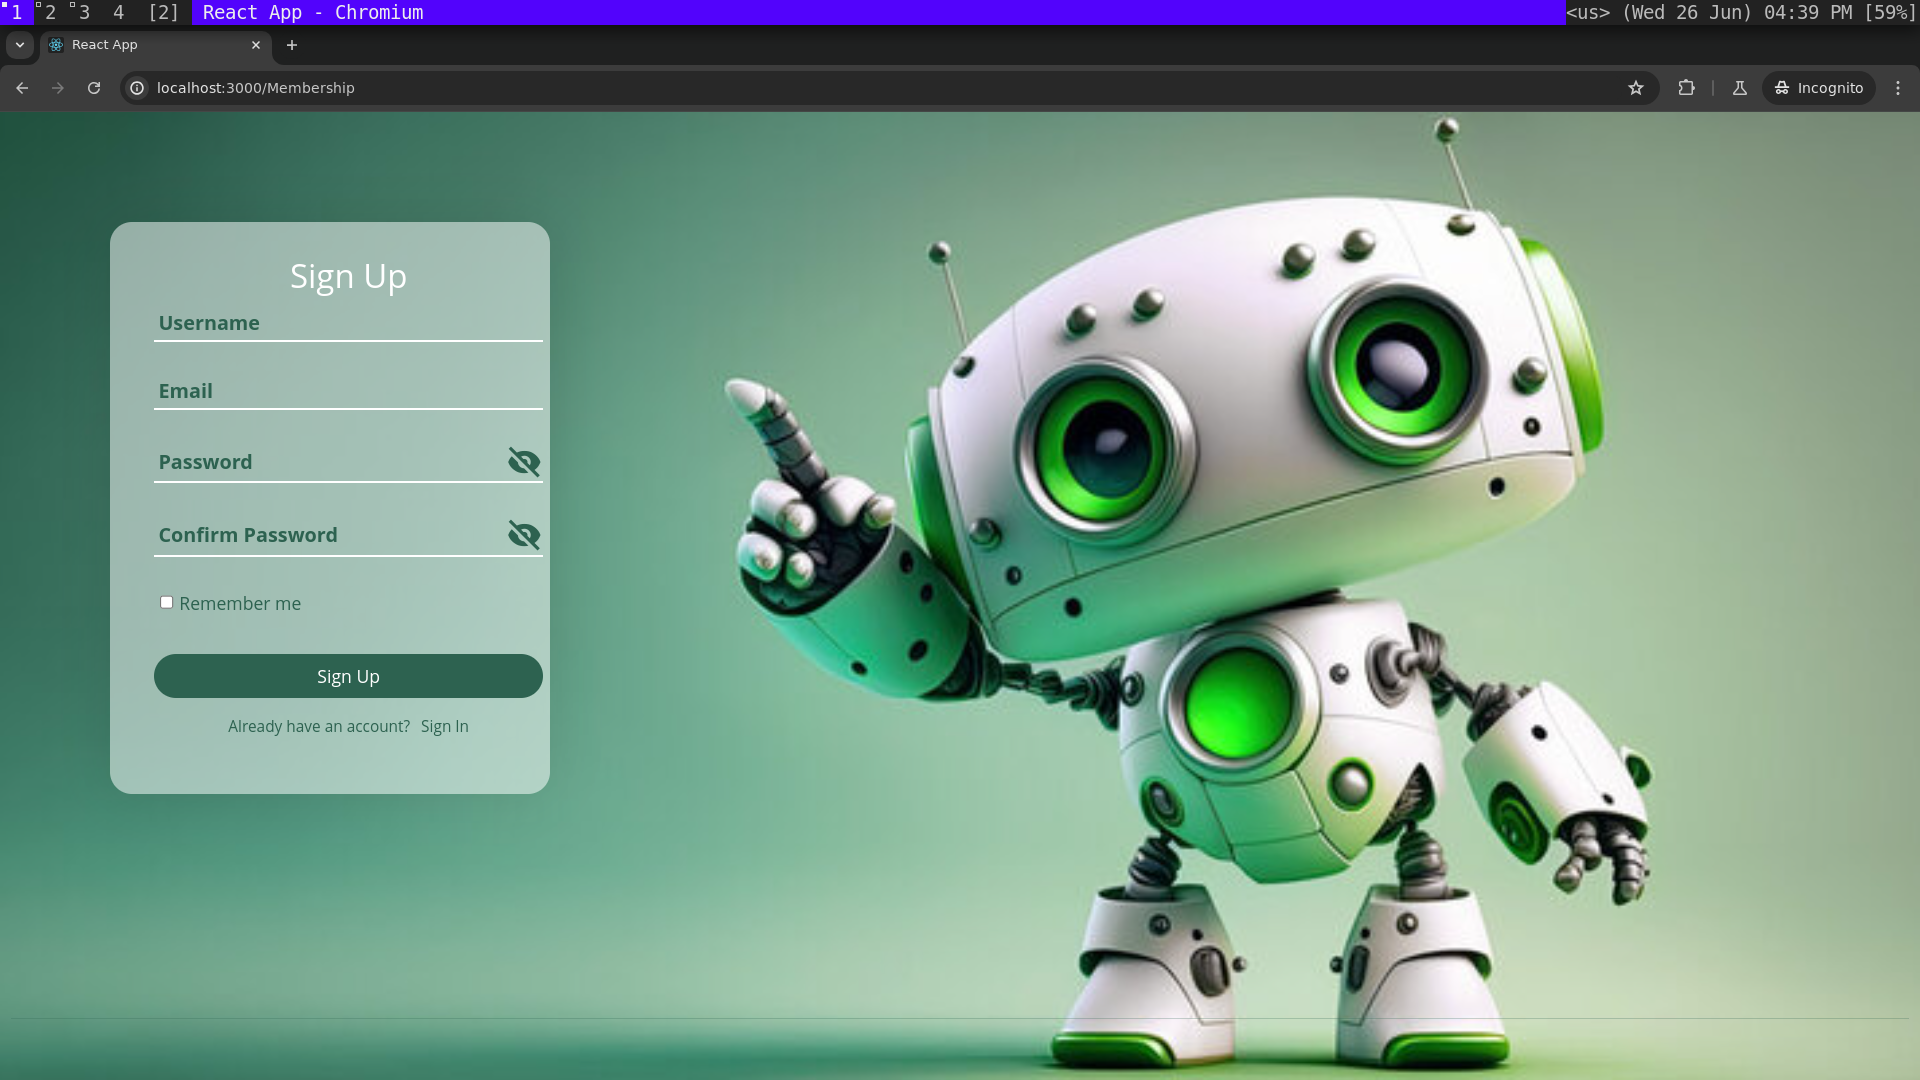
\includegraphics[scale=0.2]{./Figures/WebApp/sign-up.png}
	\caption{Sign-up screen}
	\label{fig:sign-up}
\end{figure}
\begin{figure}[h!]
	\centering
	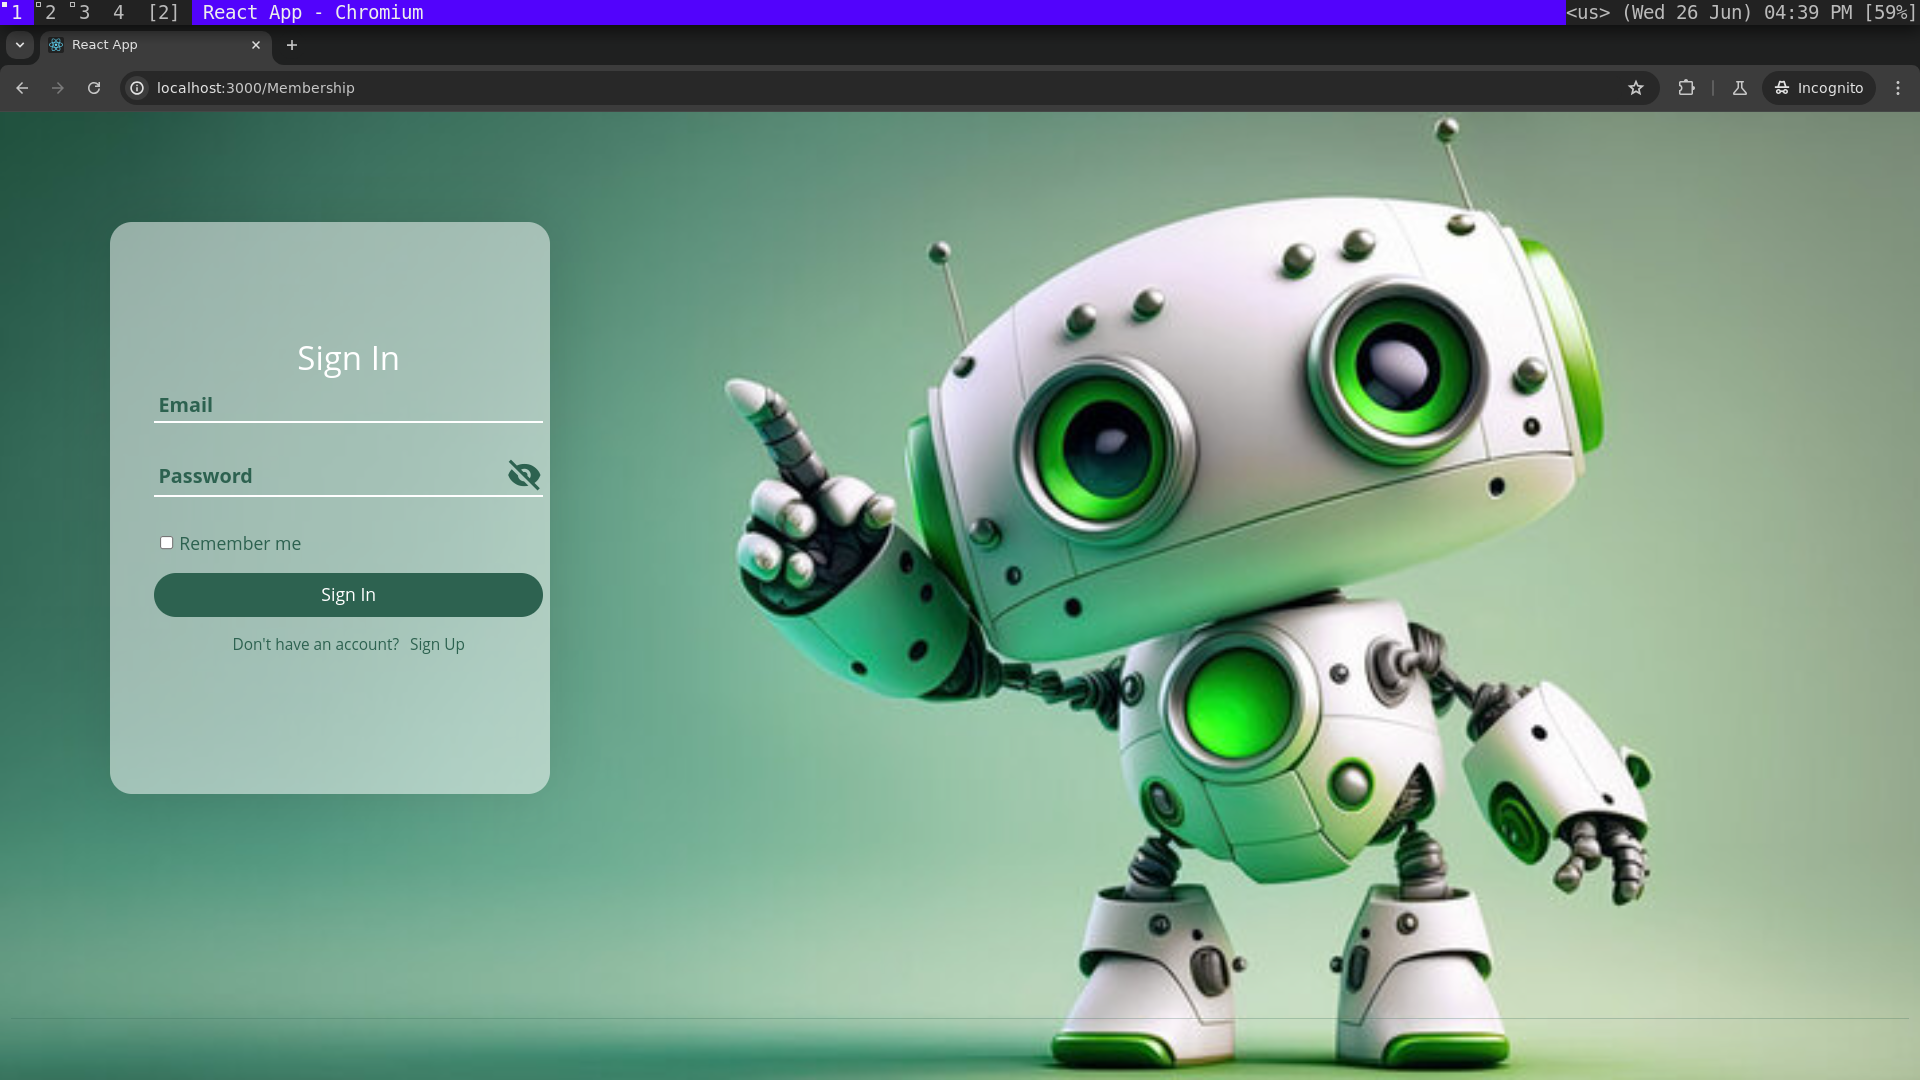
\includegraphics[scale=0.2]{./Figures/WebApp/sign-in.png}
	\caption{Sign-in screen}
	\label{fig:sign-in}
\end{figure}

\newpage

Once logged in, the user can use the home screen shown in figure \ref{fig:homePage} to navigate the web application. The typical use-case is that the user wants to create a task and assign it to a robot.

First the user must define the map in which the task will take place.Using the screen shown in figure \ref{fig:maps-management}, the user may create a new map or view predefined maps. If the user wishes to create a new map or edit a pre-existing one, they can use the map editor shown in figure \ref{fig:node-map-editor}.

Once the map is to the user's satisfaction, they can move on to task creation using the screen shown in \ref{fig:tasks-management}. Similar to the map editor, this page allows the user to create, view, edit or delete tasks. If the user chooses to create a task, they can use the screen shown in figure \ref{fig:task-creation} to specify the details of the task. Note that this window adapts according to the map that the user chooses, as the pick-up and drop-off nodes depend on the chosen map.

Now that the the task is properly defined, the last step is to assign this task to a robot. The robots management window is shown in figure \ref{fig:robots-dashboard}, using this page the user can create a new robot as shown in figure \ref{fig:create-robot}, or edit a pre-existing robot. Editing a robot is the way in which the user can assign a task to a robot.
\newpage

\chapter{Conclusion \& Future Work}

\section{Observing The Final Version}

Although the project has fulfilled most if not all of its goals, there exists many areas that can be improved and/or built upon to achieve an even greater outcome. Possible improvement ideas will be discussed in addition to recommendations for anyone willing to pick the project up where it was left off.

The proposed system proved to both be a success and come short in many areas. The project has succeeded in accomplishing most of the listed development objectives. However, the following points were not fully fulfilled or did not work as desired:
\begin{itemize}
	\item The mechanical chassis \& arm have limited weight tolerance due to the team's inexperience in mechanical design.
	\item The array of sensors used could have used a few additions like a LiDAR.
	\item The used software platform for MCU programming did not make full use of its capabilities: if the STM32 was programmed using embedded C/C++ and ran a real-time operating system it would have given a better performance.
	\item The VLC prototype is promising, but it needs to be built upon to produce a reliable product.
	\item The used stereo camera was not utilized to its full features: it is capable of depth mapping and object detection and, ultimately, could have been used in localization. It was only used for streaming in this implementation.
	\item The static map design is not always applicable. Maps tend to be more dynamic in real life.
	\item The server being a virtual machine is not portable, and a bit clunky to manage.
	\item The web application could have been developed using a framework that leverages server-side rendering with better performance than the one used.
\end{itemize} 

\newpage

\section{Future Improvements}
There are many areas to improve in each layer of the robot. It can be summarized as follows:
\begin{enumerate}
	\item Designing a better and stronger chassis equipped with a better arm.
	\item Equip the robot with a LiDAR sensor for better dynamic environment mapping.
    \item Programming all microcontrollers in embedded C/C++ and abandoning Arduino platform for a better performing system.
    \item Using a real-time operating system on all microcontrollers in order for the system to meet real-time demands.
    \item Using MicroROS---which is built on the newer architecture of ROS 2---instead of ROS 1 for a more coherent and future-proof system.
    \item Developing an embedded Linux image for the single board computer for minimum system overhead.
    \item Utilize the used stereo camera to improve localization.
    \item Containerizing the web application using Docker/Docker-Compose for more portability.
    \item To enhance the web application, we should refactor our current React and Laravel components to a Next.js framework, leveraging its server-side rendering capabilities for improved performance and SEO.
\end{enumerate}